\documentclass[
	twoside,
%	draft,
	fontsize=12pt,
	headsepline,
	cleardoublepage=empty,
	numbers=noenddot,
	bibliography=totoc,
]{scrbook}

\usepackage{ks}
\usepackage{subfigure}

% customize name, title, ...
\renewcommand{\thesisAuthor}{Julian Daberkow\\Julian Exner\\Andreas Gatting\\Timo Michalski\\Hendrik Oestreich}
\renewcommand{\thesisStudNum}{1234567}
\renewcommand{\thesisTitle}{Autonomes Ladeverhalten für den AMiRo\\im Rahmen eines Fußballszenarios }
\renewcommand{\thesisDate}{Bielefeld, März 2016}
\renewcommand{\thesisId}{}
\renewcommand{\thesisType}{Projektbericht}
\renewcommand{\thesisCourse}{Autonomous Systems Engineering}
\renewcommand{\thesisSupervisor}{M.Sc.~Timo~Korthals\\M.Sc.~Thomas~Schöpping}

% hyphenation
\hyphenation{
Pro-zes-sor-e-le-men-te
Pro-zes-sor-e-le-men-ten
Pro-zes-sor-e-le-men-tes
}

\begin{document}
\pagenumbering{roman}
\begin{titlepage}
\fontfamily{phv}
\fontseries{m}
\selectfont
\leftskip2em

\begin{minipage}[t]{0.4\textwidth}
\large \thesisType\\
\normalsize \thesisCourse
\end{minipage}
\hfill
\begin{minipage}[t]{0.4\textwidth}
\begin{flushright}
CITEC, Universität Bielefeld\\
AG Kognitronik \& Sensorik \\
Prof. Dr.-Ing. Ulrich Rückert     
\end{flushright}
\end{minipage}

\vfill

{\fontfamily{phv}\fontseries{bc}\selectfont 
\Huge \thesisTitle
\begin{flushright}
\Large \thesisAuthor
\end{flushright}
}

\vfill

\normalsize
%\begin{minipage}[t]{5em}
%Matr.-Nr.:\quad
%\end{minipage}
%\begin{minipage}[t]{0.5\textwidth}
%\thesisStudNum
%\end{minipage}

\begin{minipage}[t]{5em}
Betreuer:\quad
\end{minipage}
\begin{minipage}[t]{0.5\textwidth}
\thesisSupervisor
\end{minipage}




\vfill

\thesisDate
\hfill
\thesisId

% enlarge page by 2 lines
\enlargethispage{2\baselineskip}

\end{titlepage}

\cleardoublepage
\subsection*{Kurzfassung}

Um autonome Paradigmen für Miniroboter in einem größeren Zeitfenster etablieren zu können, wird eine autark bewerkstelligte Energieversorgung benötigt. In der vereinfachten Welt des Schaukastens wurden in diesem Projekt dafür die Lokalisation der Ladestation, das Anfahren und Einparken sowie das Andocken an den Lademechanismus realisiert. Zur Einbettung in einen anwendungsorientieren Kontext wurde zudem ein Fußballszenario implementiert, in dem zwei AMiRos gegeneinander antreten. Dabei wird das Szenario extern überwacht und spielentscheidende Elemente werden identifiziert und visualisiert. 


\tableofcontents

%% content
\cleardoublepage
\pagenumbering{arabic}

\chapter{Einleitung} \label{kap:einleitung} %TODO: Wer?
- Bezug nehmen auf Vorlesungsinhalte --> Übertragung auf realisiertes Projekt

- Ziele und Voraussetzungen einarbeiten:\\
Ziele:\\
Fußball Tipp-Kick Szenario \\
Autonome Ladestrategien für AMiRos\\
Spieltracking durch Bildverarbeitung\\
\\
Voraussetzungen:\\
2 AMiRos\\
1 Ladestation\\
1 Schaukasten\\
1 Webcam\\
1 Host-PC\\
1 Router\\
2 Tore\\
1 Spielball\\
diverse AR-Marker\\

%TODO: 
Beschreibung der Kapitelautoren?
z.B. Hendrik Oestreich = H.O.
(siehe Beispielhafte Formatierung Section Szenario Koordination)
Funktioniert mit dem Kommando \texttt{sectionauthor} . Erfordert manuelles Einfügen eines \texttt{vfill} Kommandos bei der abschließenden Formatierung der Seiten.
\chapter{Autonomes Ladeverhalten} \label{kap:AutonomesLadeverhalten}

\section[Anfahren der Ladestation]{Anfahren der Ladestation\hfill {\normalsize A.G.}} \label{cha:Anfahren der Ladestation} %TODO: Andi G.

Damit der AMiRo sich in der Ladestation aufladen kann, muss diese zunächst lokalisiert und angefahren werden. Hierbei dient der komplette Schaukasten als Bewegungsfläche und der Schaukastenrand als Begrenzung dieser Fläche. Für die Suche kann der AMiRo auf unterschiedliche Strategien und Verfahren zurückgreifen. Als Suchstrategien existiert zum einen eine Positionsabschätzung über die Kamerabilder der Umgebung, um den kürzesten Pfad zum Schaukastenrand zu berechnen. Zum anderen kann der AMiRo sich in die aktuelle Richtung bewegen und auf gut Glück den Schaukastenrand finden. Als Verfahren zum Anfahren der Ladestation wird entweder auf die Kamera oder auf die Infrarotsensoren am Boden des AMiRo's zurückgegriffen.

In der Abbildung \ref{fig:searchStationFSM} ist die Finite-State-Machine der Lokalisation und des Anfahren der Ladestation aufgeführt. Diese lokale State-Machine wird durch die globale Finite-State-Machine angestoßen, welche im Abschnitt \ref{cha:Finite-State-Machine} vorgestellt wird. In der Abbildung wird diese als \texttt{showcaseFSM} beschrieben. Wird das Anfahren der Ladestation aktiviert, beginnt es zunächst aus dem Zustand \texttt{Idle}. Mit der Aktivierung wird eine Information zum weiteren Verlauf mitgegeben. Entweder soll sich der AMiRo zum Schaukastenrand bewegen oder die Ladestation anfahren. Letzteres wird ausgeführt, wenn sich der AMiRo bereits am Schaukastenrand befindet. Dort muss er bei eventuell besetzter Ladestation warten. Aus diesem Grund kann diese lokale State-Machine in zwei Kernabschnitte betrachtet werden, die in der Abbildung als rote Kästen dargestellt sind. Ein beispielhaftes Szenario ist in Abbildung \ref{fig:searchStationExample} visualisiert, wobei der rote Pfeil zum Schaukastenrand den ersten Kernabschnitt und der rote Pfeil zur Ladestation den zweiten Kernabschnitt repräsentiert.

\begin{figure}[H]
	\begin{center}
		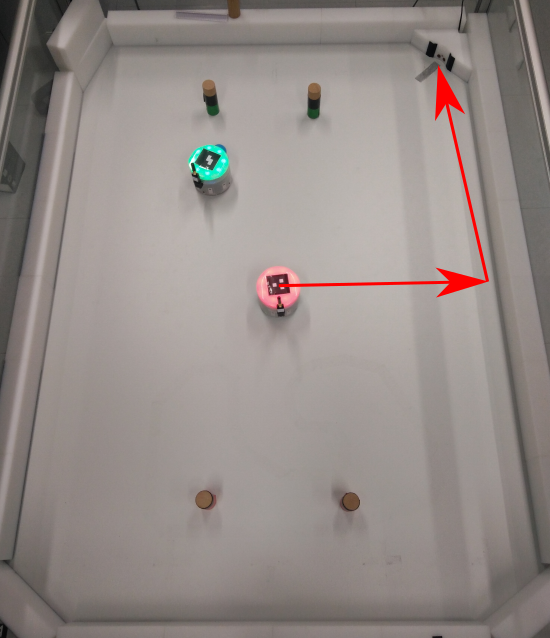
\includegraphics[scale=.45]{searchSationExample.png} 	
		\caption{Aufsuchen der Ladestation}
		\label{fig:searchStationExample}
	\end{center}
\end{figure}

Im ersten Kernabschnitt (oberer roter Kasten in Abb. \ref{fig:searchStationFSM}) soll sich der AMiRo zum Schaukastenrand bewegen. Dabei ruft der Zustand \texttt{Idle} den Zustand \texttt{Initialization} auf. Hier werden für das Lokalisieren und Anfahren Parameter initialisiert und entschieden, welche Suchstrategie ausgeführt wird. Soll der AMiRo lediglich in seine aktuelle Orientierung fahren, wird ohne Weiteres der Zustand \texttt{moveAndCollAvoid} aufgerufen. Hierbei fährt er in seine aktuelle Orientierung bis die Kollisionsvermeidung greift. 

Soll hingegen eine intelligentere Suchstrategie angewendet werden, wechselt die State-Machine in den Zustand \texttt{checkPosition}. Der AMiRo rotiert hier einmalig vollständig um seine eigene Achse, während Kamerabilder von der Umgebung aufgenommen werden. Über die Bilder läuft der \textit{SimpleBlobDetector} der OpenCV-Programmbibliothek, wobei das Bild zunächst vorverarbeitet wird. Bei der Vorverarbeitung wird pixelweise entschieden, ob der aktuelle Bildpunkt in einem bestimmten Farbwertrahmen fällt oder nicht. Bei zutreffender Bedingung behält der Pixel seinen Farbwert, andernfalls wird er weiß eingefärbt. Damit bietet es dem \textit{SimpleBlobDetector} eine kontrastreiche Vorlage, um Elemente im Kamerabild zu detektieren. Wurde ein Torpfostenpaar und optional die Ladestation detektiert, werden zum einen jeweils die Orientierung der Odometrie gespeichert. Zum anderen werden jeweils Minimum und Maximum der X- und Y-Koordinate beider Torpfosten errechnet. Mit diesen Informationen wechselt die State-Machine in den Zustand \texttt{goalDetected}, ansonsten direkt in den Zustand \texttt{moveAndCollAvoid}.

\begin{figure}[H]
	\begin{center}
		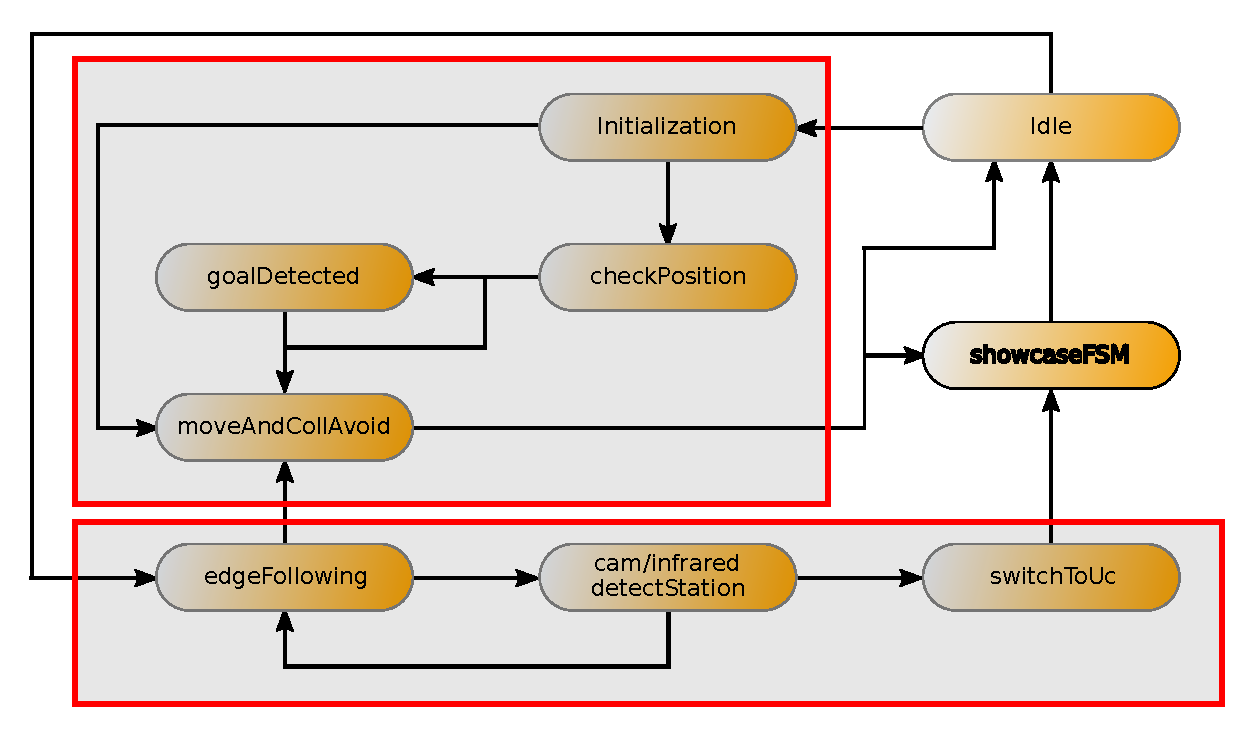
\includegraphics[scale=.7]{searchStationFSM.pdf} 	
		\caption{Finite-State-Machine zur Lokalisation der Ladestation}
		\label{fig:searchStationFSM}
	\end{center}
\end{figure}

Das Vorgehen zur Berechnung der nächsten Kante in \texttt{goalDetected} wird in Abschnitt \ref{cha:Lokalisation der Ladestation} erläutert. Nachdem sich der AMiRo zur nächsten Kante orientiert hat, wird ebenfalls der Zustand \texttt{moveAndCollAvoid} aufgerufen. In diesem Zustand bewegt sich der AMiRo geradeaus, entweder eine definierte oder unbegrenzte Strecke. Im ersteren Fall wird eine neue Position angefahren, da die Detektion der Torpfosten an der alten Position nicht erfolgreich war. Damit wechselt die State-Machine in den Zustand \texttt{Idle} und beginnt von vorne. Die Anzahl der Versuche ist hierbei einstellbar, sodass der AMiRo zur Not die aktuelle Orientierung anfährt. Dies entspricht dem zweiten Fall, der unbegrenzten Strecke. Mit einer Kollisionsvermeidung wird anschließend das aktuelle Hindernis vorerst als Schaukastenrand interpretiert. Damit endet der erste Kernabschnitt der lokalen State-Machine und sendet ein Signal an die \texttt{showcaseFSM}.

Der zweite Kernabschnitt (unterer roter Kasten in Abb. \ref{fig:searchStationFSM}) befasst sich mit dem Anfahren der Ladestation. Dazu wird ausgehend vom Zustand \texttt{Idle} mit der Information der \texttt{showcaseFSM} der Zustand \texttt{edgeFollowing} angestoßen. Die durchzuführende Kantenverfolgung ist in Abbildung \ref{fig:edgeFollowing} dargestellt. Ausgehend von einer erfolgreichen Detektion der Ladestation im ersten Kernabschnitt, wird zunächst die Richtung der Kantenverfolgung gesetzt. Das bedeutet den kürzesten Pfad zur Ladestation entweder im oder gegen den Uhrzeigersinn. Des weiteren wird mithilfe der Infrarotsensoren seitlich am AMiRo versucht einen bestimmten Abstand zum Schaukastenrand einzuhalten. Hierbei wird permanent überprüft, ob die Sensoren einen minimalen oder maximalen Schwellwert überschreiten. Trifft dies zu, wird ein entsprechender Rotationswert (links/rechts) angelegt. Befindet sich der Sensorwert zwischen min. und max. Schwellwert, bewegt sich der AMiRo geradeaus. Parallel wird dazu die Orientierung der Odometrie zur Kantenüberprüfung aufsummiert. Erreicht die Summe einen zu hohen Wert, befindet sich der AMiRo nicht an der Kante, da die Innenwinkelsumme eines Rechteckes $360^\circ$ beträgt. Damit wechselt der Miniroboter zurück zum Zustand \texttt{moveAndCollAvoid} und sucht ein neues Hindernis bzw. Kante.

Nachdem (für den Moment) Motorwerte zur Kantenverfolgung eingestellt sind, wechselt die State-Machine in den Zustand \texttt{cam/infrared detectStation}. An dieser Stelle wird ein Verfahren zur Detektion der Ladestation verwendet, mittels Kamera oder Infrarotbodensensoren.

\begin{figure}[H]
	\begin{center}
		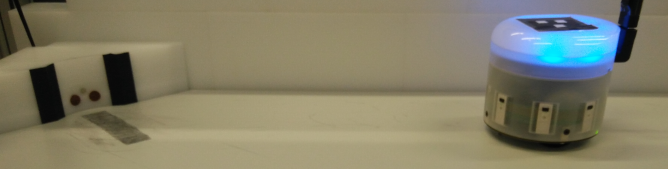
\includegraphics[scale=.6]{edgeFollowing.png} 	
		\caption{Kantenverfolgung und Anfahren der Ladestation}
		\label{fig:edgeFollowing}
	\end{center}
\end{figure}

Die Detektion über das Kamerabild verläuft sehr ähnlich zur Detektion der Torpfosten im ersten Kernabschnitt. Wiederholt wird das Kamerabild vorverarbeitet und der \textit{SimpleBlobDetector} zur Erkennung der schwarzen Markierungen der Ladestation verwendet. Sind keine passenden Elemente detektiert worden, wechselt die State-Machine zurück in den Zustand \texttt{edgeFollowing}. Dies geschieht solange in einer Schleife, bis beide schwarzen Markierungen detektiert worden sind. Ab diesem Punkt richtet sich der AMiRo mit dem Bildmittelpunkt (X-Achse) zur Ladestation aus und fährt sie direkt an. Weiterhin im aktuellen Zustand verweilend, wird durchgängig über die seitlichen Infrarotsensoren der Abstand vor dem Miniroboter überprüft. Durch die Überschreitung eines Schwellwertes befindet sich der AMiRo in der Ladestation und wechselt zum Zustand \texttt{switchToUc}.

Ein zweites Verfahren ist die Detektion über die Infrarotbodensensoren. In Abbildung \ref{fig:edgeFollowing} ist eine schwarze Bodenmarkierung an der Ladestation ersichtlich. Wie bei der Detektion mit dem Kamerabild, wechselt die State-Machine solange zwischen diesem Zustand und dem Zustand \texttt{edgeFollowing}, bis die Infrarotsensoren am Boden einen Schwellwert überschreiten. An dieser Stelle wird die Geschwindigkeit gedrosselt und der AMiRo richtet sich zur Ladestation aus. Sobald die seitlichen Bodensensoren die schwarze Fläche detektieren, wird der Miniroboter nochmals zur Ladestation ausgerichtet. Des weiteren bewegt er sich langsam zur Station und sobald die vorderen (Ringsensoren) einen Schwellwert überschreiten, befindet sich der AMiRo in der Ladestation und wechselt zum Zustand \texttt{switchToUc}.

Der Zustand \texttt{switchToUc} ist der finale Zustand in dieser State-Machine. Hier werden Parameter zurückgesetzt und das erfolgreiche Anfahren der Ladestation durch Lichter visualisiert. Ein Signal an \texttt{showcaseFSM} beendet den zweiten Kernabschnitt.

\section[Lokalisation der Ladestation durch Positionsabschätzung]{Lokalisation der Ladestation durch Positionsabschätzung\hfill {\normalsize A.G.}} \label{cha:Lokalisation der Ladestation}
Da der Begriff \textit{autonom} ein gewisses intelligentes Verhalten für die Selbstständigkeit mit sich zieht, ist eine zufällige Suche der Ladestation nicht optimal. Aus einer Menge vieler möglichen Strategien wurde die Berechnung der nächsten Kante und die darauffolgende kürzeste Strecke zur Ladestation gewählt. Diese Strategie lässt sich gut über das Kamerabild realisieren und bietet durch die Aufteilung eine Robustheit mit der Annahme, dass die Ladestation durch eine Kantenverfolgung erreicht werden kann.

Da im Schaukasten hinsichtlich der Markierungen sehr minimalistisch gearbeitet wurde, ist eine Positionsabschätzung anhand der Torpfosten eine gute Möglichkeit. Alternativ wäre eine interne Karte eine weitere Möglichkeit, allerdings ist dies im Rahmen dieses Projektes zu viel Aufwand.

Mit der Bestimmung des nächsten Torpfosten beginnt der Zustand \texttt{goalDetected}. Grundlage dafür sind die über den \textit{SimpleBlobDetector} jeweils ermittelten minimalen und maximalen X- und Y-Koordinaten der Torpfosten. Mit der Annahme, dass Objekte mit zunehmender Entfernung zum Betrachter kleiner wirken, wird der nächste Torpfosten anhand der relativen Größe bestimmt. Diese Information ist im späteren Verlauf für die endgültige Ausrichtung wichtig. Als nächstes folgt die vorläufige Drehung zum Tor, um die einzelnen Schritte zu visualisieren. Dies wird in der Abbildung \ref{fig:firstRotationToPost} dargestellt. Die Orientierung der Odometrie zum Tor wurde in der vorherigen Detektion der Torpfosten mit abgespeichert (rote, gestrichelte Linie). Der Differenzwinkel $\Delta_\Theta$ wird demnach aus dieser und der Orientierung der Startposition berechnet.

\begin{figure}[h]
	\begin{center}
		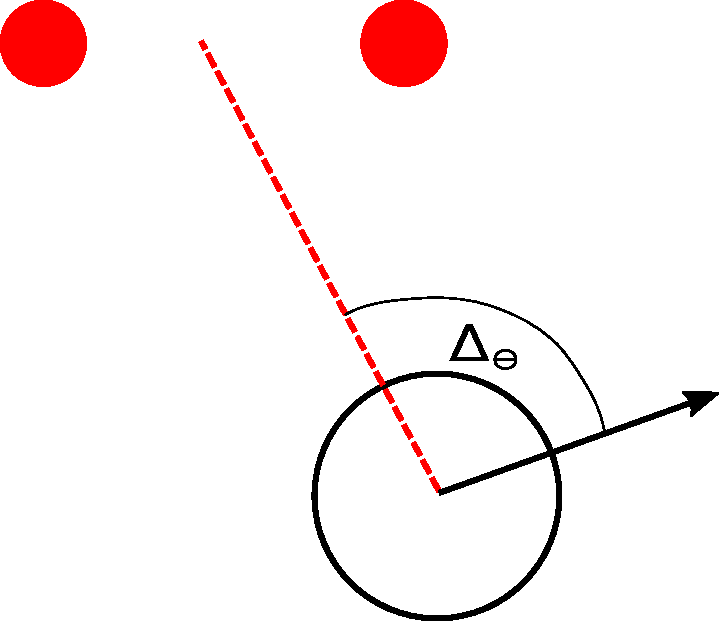
\includegraphics[scale=.6]{firstRotationToPost.pdf} 	
		\caption{Ausrichtung des AMiRo zum Tor}
		\label{fig:firstRotationToPost}
	\end{center}
\end{figure}

Mit den statischen Informationen (Position und Dimensionen), können die Torpfosten als Landmarken im Raum verwendet werden. Die Schaukastendimensionen dienen dazu als Koordinatensystem, um eine Positionsabschätzung zu liefern. Dafür werden im folgenden die Distanzen zu den Torpfosten und die Winkel zu diesen benötigt, die mittels Trigonometrie berechnet werden.

Die Distanzberechnung zum Torpfosten ist schematisch in Abbildung \ref{fig:distToPost} dargestellt. Hierbei ist der Winkel $\Theta$ der halbe vertikale Kamerawinkel, da im gesamten Verlauf die relevanten Objekte unterhalb des Horizontes liegen und nur das untere Kamerabild betrachtet wird. Dies spart zum einen Rechenleistung bei der Bildanalyse und zum anderen reduziert es potentiell falsche Objektdetektion. Um die Gegenkathete $B$ zu erhalten, wird die statische Größe des Torpfostens auf die vertikale Bildgröße hochskaliert. Mit Winkel $\Theta$ und Gegenkathete $B$ wird in der Gleichung \ref{eq:distanceToPost} die Ankathete bzw. Distanz $A$ bestimmt.

\begin{equation}
	A = B \cdot \tan(\Theta)
	\label{eq:distanceToPost}
\end{equation}

\begin{figure}[h]
	\begin{center}
		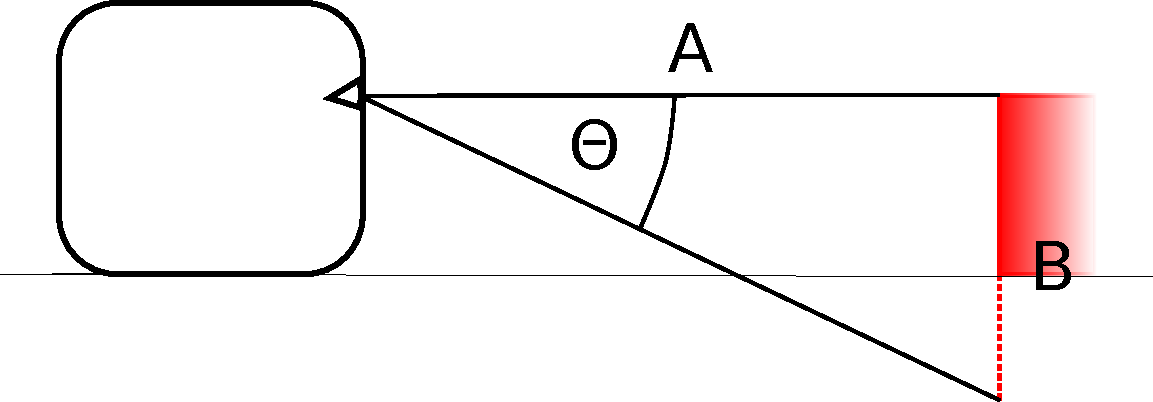
\includegraphics[scale=.6]{distanceToPost.pdf} 	
		\caption{Distanzberechnung zum Torpfosten}
		\label{fig:distToPost}
	\end{center}
\end{figure}

Für die Berechnung der Positionswinkel zu dem Torpfosten wird der Kosinussatz verwendet. Hierzu sind in Abbildung \ref{fig:trianglePost} die zuvor berechneten Distanzen zu den Torpfosten als Ankathete $B$ und Hypotenuse $C$ zu sehen. Der Gegenkathete $A$ ist der Abstand zwischen den Torpfosten und somit eine bekannte Konstante. Mit den drei Seiten können alle Winkel des Dreiecks über den Kosinussatz, den Gleichungen in \ref{eq:anglePost}, berechnet werden. Der relevante Positionswinkel ist hier die Summe $\epsilon = \alpha + \beta$. Steht der AMiRo linksseitig vom Tor, wäre die Winkelsumme $\epsilon = \alpha + \gamma$ (nächster Torpfosten, siehe oben). 

\begin{equation}
	\begin{aligned}
		\alpha = \arccos(\frac{B^2 + C^2 - A^2}{2 \cdot B \cdot C}) \\\\
		\beta = \arccos(\frac{A^2 + C^2 - B^2}{2 \cdot A \cdot C}) \\\\
		\gamma = \arccos(\frac{A^2 + B^2 - C^2}{2 \cdot A \cdot B})
		\label{eq:anglePost}
	\end{aligned}
\end{equation}

\begin{figure} []
	\subfigure[Winkelberechnung]{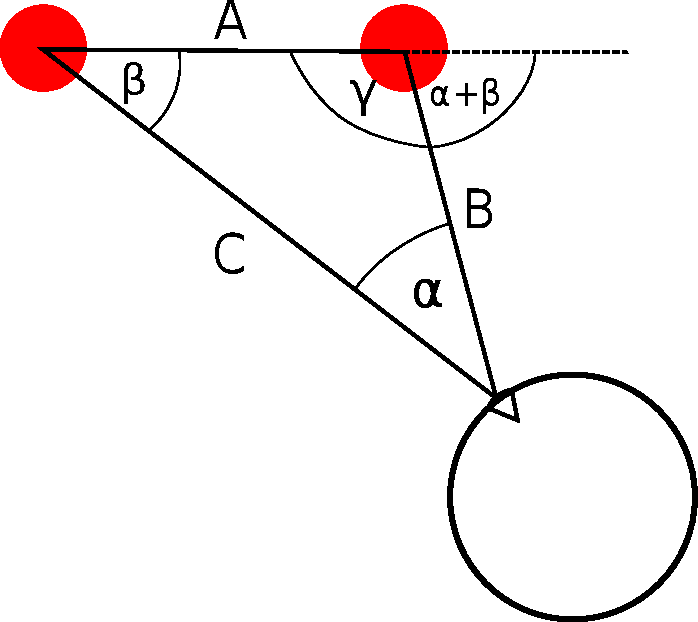
\includegraphics[width=0.4\textwidth]{trianglePost.pdf}\label{fig:trianglePost}} \hspace{2cm}
	\subfigure[Koordinatenberechnung]{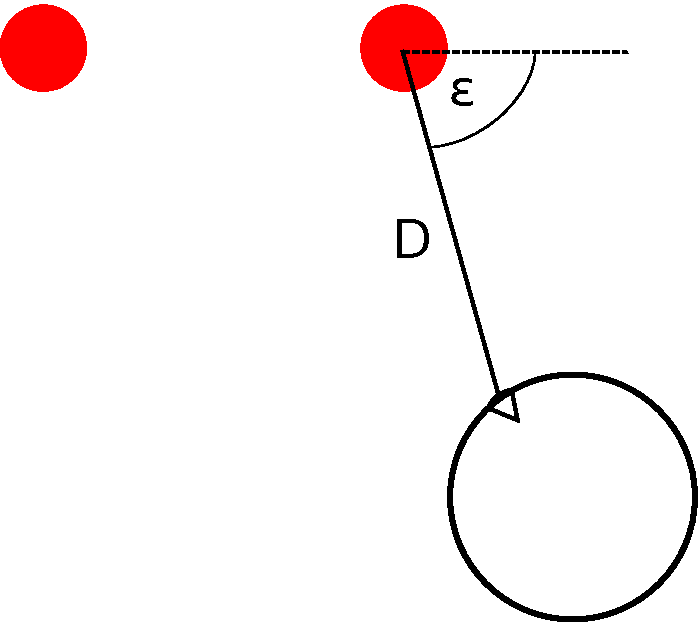
\includegraphics[width=0.4\textwidth]{coordsAmiro.pdf}\label{fig:coordsAmiro}} 
	\caption{Winkel- und Koordinatenberechnung des AmiRo} 
	\label{fig:triangleAndCoordsPost}
\end{figure}

Durch die hinzugekommenen Distanz- und Winkelinformation ist nun eine Positionsabschätzung möglich. In Abbildung \ref{fig:coordsAmiro} sind diese eingezeichnet. Die beiden Gleichungen in \ref{eq:positionCoords} beschreiben die Berechnung der X und Y Koordinaten mit $D$ als Distanz und $\epsilon$ als Winkel. Abhängig von der Position des AMiRos zum nächsten Torpfosten, linksseitig oder rechtsseitig, wird der Wert zur Torposition addiert oder subtrahiert.

\begin{equation}
	\begin{aligned}
		x\_amiro = x\_tor~+-~~D \cdot \cos(\epsilon) \\\\
		y\_amiro = y\_tor~+-~~D \cdot \sin(\epsilon)
		\label{eq:positionCoords}
	\end{aligned}
\end{equation}

Mit der Positionsabschätzung lässt sich im weiteren die nächste Kante identifizieren. In der Abbildung \ref{fig:showcaseSplit} ist die Aufteilung der Fläche des Schaukastens ersichtlich. Jedes Gebiet beschreibt dabei die Richtung zur nächsten Kante, welche durch die vier großen Pfeile in der Abbildung verdeutlicht wird. Da der Schaukasten als Koordinatensystem angesehen wird und dem AMiRo eine Positionsabschätzung mit Koordinaten zugeordnet wurde, kann das aktuelle Gebiet ermittelt werden. Der Positionswinkel $\epsilon$ wird hier als Grundlage zur Ausrichtung zur nächsten Kante eingesetzt. Dieser Winkel $\epsilon$ beschreibt in diesem Szenario immer ein Drehwinkelverhältnis zu einem der seitlichen Kante. Das bedeutet den tatsächlichen Drehwinkel $\Delta_\Theta = 180 - \epsilon$, welcher dem Winkel $\gamma$ aus der Abbildung \ref{fig:trianglePost} entspricht. In $90^\circ$-Schritten wird der Drehwinkel für die anderen Kanten ausgerechnet. Nach der Bestimmung des Drehwinkels, richtet sich der AMiRo aus und die State-Machine aus Abschnitt \ref{cha:Anfahren der Ladestation} wechselt in den Zustand \texttt{moveAndCollAvoid}.

\begin{figure}[h]
	\begin{center}
		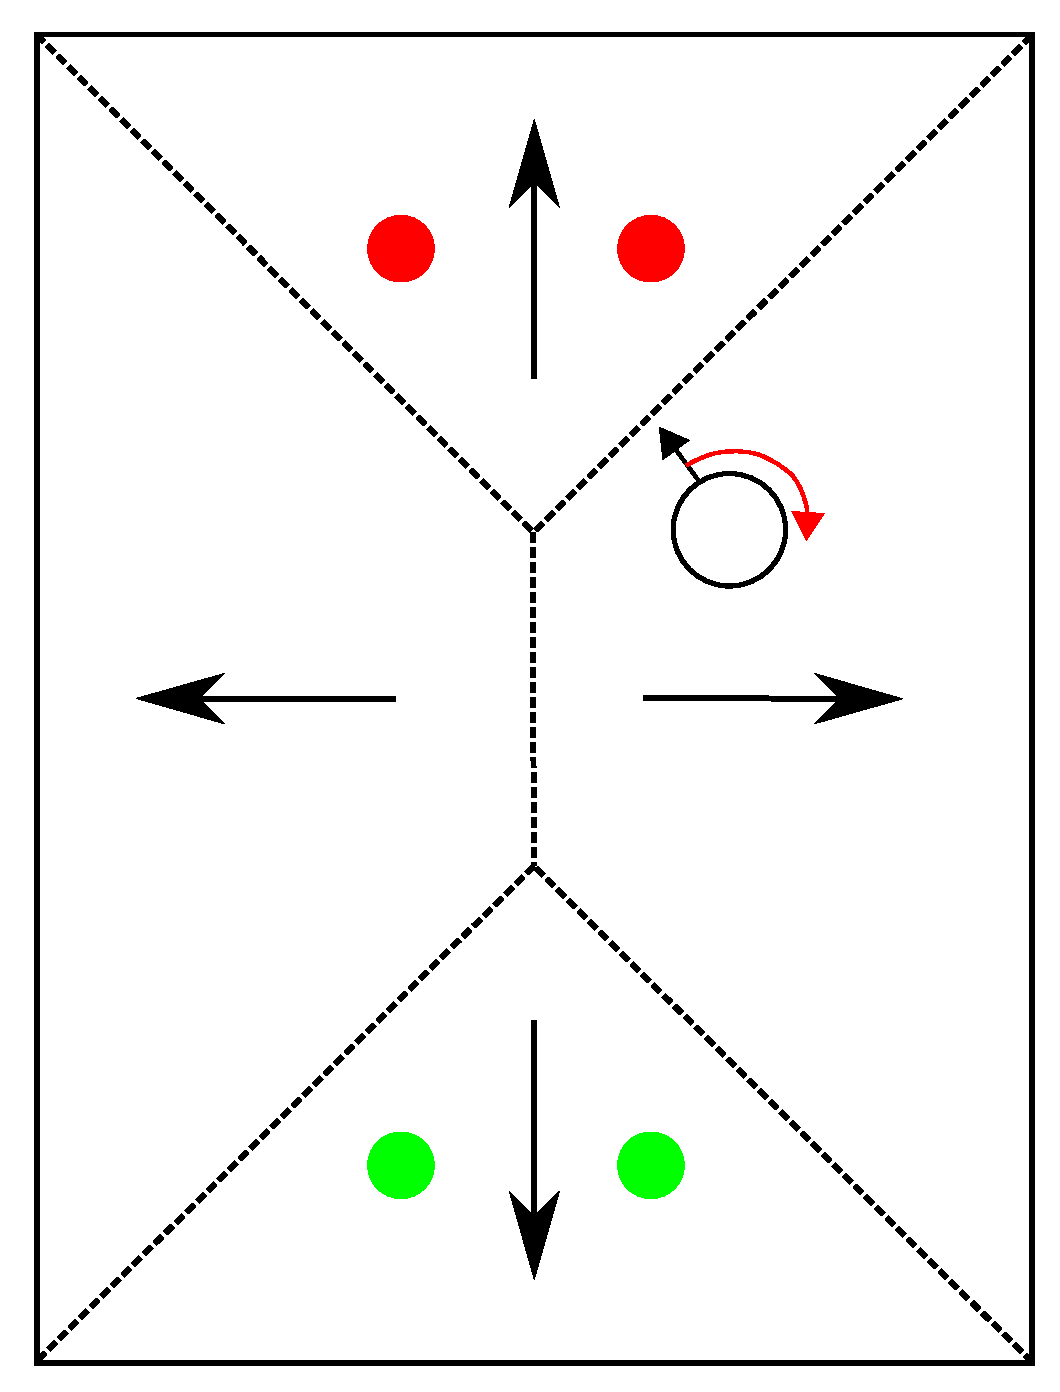
\includegraphics[scale=.4]{showcaseSplit.pdf} 	
		\caption{Gebietsaufteilung im Schaukasten}
		\label{fig:showcaseSplit}
	\end{center}
\end{figure}

\section[Finite-State-Machine des DiWheelDrive-Microcontrollers]{Finite-State-Machine des DiWheelDrive-Microcontrollers\hfill {\normalsize J.E. \& T.M.}} %TODO: Julian E. & Timo M.

Nachdem die Ladestation erfolgreich angefahren wurde, wird durch eine CAN-Nachricht dem DiWheelDrive-Board signalisiert, dass die weiteren Schritte des Einparkens eingeleitet werden sollen.
Auf dem Microcontroller wird eine State-Machine ausgeführt, die so lange im \textit{IDLE}-Zustand wartet, bis das Ladeverhalten angetriggert wird (siehe Abb. \ref{fig:uC_statmachine}).
Der nächste Zustand ist \textit{MOVE INTO STATION}, welcher in Kapitel \ref{kap:einparken_ladestation} erläutert wird. Ist dies erfolgreich abgeschlossen, so folgen die Zustände \textit{TURN AROUND} und \textit{ADJUST POSITION}, welche in Kapitel \ref{kap:andocken_ladestation} erklärt werden. Anschließend wird der Ladevorgang des AMiRos gestartet und überwacht. Dies geschieht in den Zuständen \textit{INITIATE CHARGING} und \textit{CHARGING}. Diese sind im Kapitel \ref{kap:ladevorgang} beschrieben.

Sollte ein Zustand nicht erfolgreich ausgeführt werden können, so gibt es definierte Routinen, die abermals ausgeführt werden müssen. Sollte die CAN-Nachricht für einen Abbruch des Ladevorganges eingehen, so wird dieser sofort unterbrochen und die State-Machine wird in den \textit{IDLE}-Zustand versetzt.

\begin{figure}[H]
	\begin{center}
		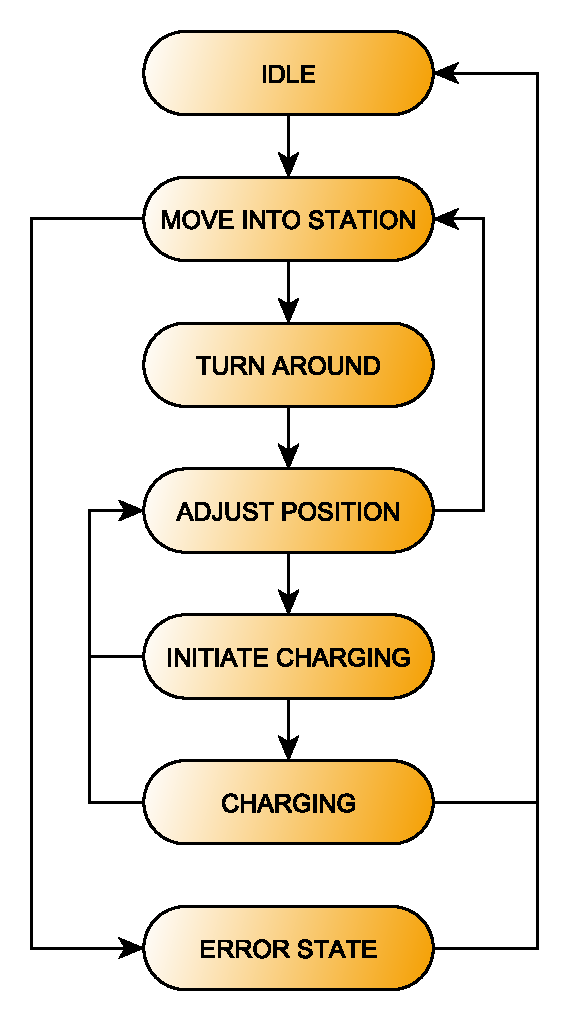
\includegraphics[width=0.4\textwidth]{uC_statemachine.pdf} 	
		\caption{Finite-State-Machine des DiWheelDrive-Microcontrollers}
		\label{fig:uC_statmachine}
	\end{center}
\end{figure}

\section[Einparken in der Ladestation]{Einparken in der Ladestation\hfill {\normalsize J.E.}}\label{kap:einparken_ladestation} %TODO: Julian E.

\section[Andocken an die Ladestation]{Andocken an die Ladestation\hfill {\normalsize T.M.}}\label{kap:andocken_ladestation} %TODO: Timo M.
Nachdem der AMiRo erfolgreich in der Ladestation eingeparkt ist werden anschließend die Ladepins auf der Rückseite des Roboters zu den Ladekontakten der Station ausgerichtet. Dabei ist es notwendig, dass alle Pins die Kontakte berühren, da es bei Stromspitzen sonst zu Schäden am AMiRo kommen könnte.

Als ersten Schritt wird zunächst eine 180$^\circ$ Drehung durchgeführt, durch die der AMiRo grob in die Ladeposition gedreht wird. Die Drehung wird anhand der Odometriedaten des Roboters durchgeführt. Dabei kann eine gewünschte Fehlertoleranz als Argument übergeben werden. Da eine exakte Drehung um 180$^\circ$ kompliziert ist, wird hier eine Fehlertoleranz von 5$^\circ$ eingeräumt, damit die Drehung schnell durchgeführt werden kann und der AMiRo nicht die Position mehrfach verbessern muss, bis exakt 180$^\circ$ erreicht sind. Diese Toleranz hat auf das anschließende Justieren der Position keine Auswirkungen.

Für die Justierung der Ladeposition des AMiRos werden die Daten der beiden hinteren Abstandssensoren genutzt. Um diese zur Ausrichtung des Roboters nutzen zu können, wurden an der Station zwei schwarze Streifen angebracht (siehe Abb. \ref{fig:charging_station}). Diese bieten einen hohen Kontrast für die UV-Sensoren im Vergleich zur weißen Station. So liefern die Sensoren den maximalen Wert von 0xFFFF, wenn sie sich direkt vor der weißen Ladestation befinden und einen im Vergleich sehr niedrigen Wert von unter 0x2000, wenn sie den Abstand zu einen schwarzen Klebestreifen messen. 
Die Klebestreifen sind so angebracht, dass sich beide hinteren Abstandssensoren genau vor einer weißen Fläche befinden, wenn die Ladeposition erreicht ist. 
Das heißt, dass die Position des AMiRos so lange justiert werden muss, bis beide Sensoren den Wert 0xFFFF liefern. 
Dafür werden die Werte der Abstandssensoren ausgelesen und anhand dieser wird nun unterschieden in welcher Position sich der AMiRo befindet und welches der nächste Schritt ist, um die Ladeposition zu erreichen. 

\begin{figure}[]
	\begin{center}
		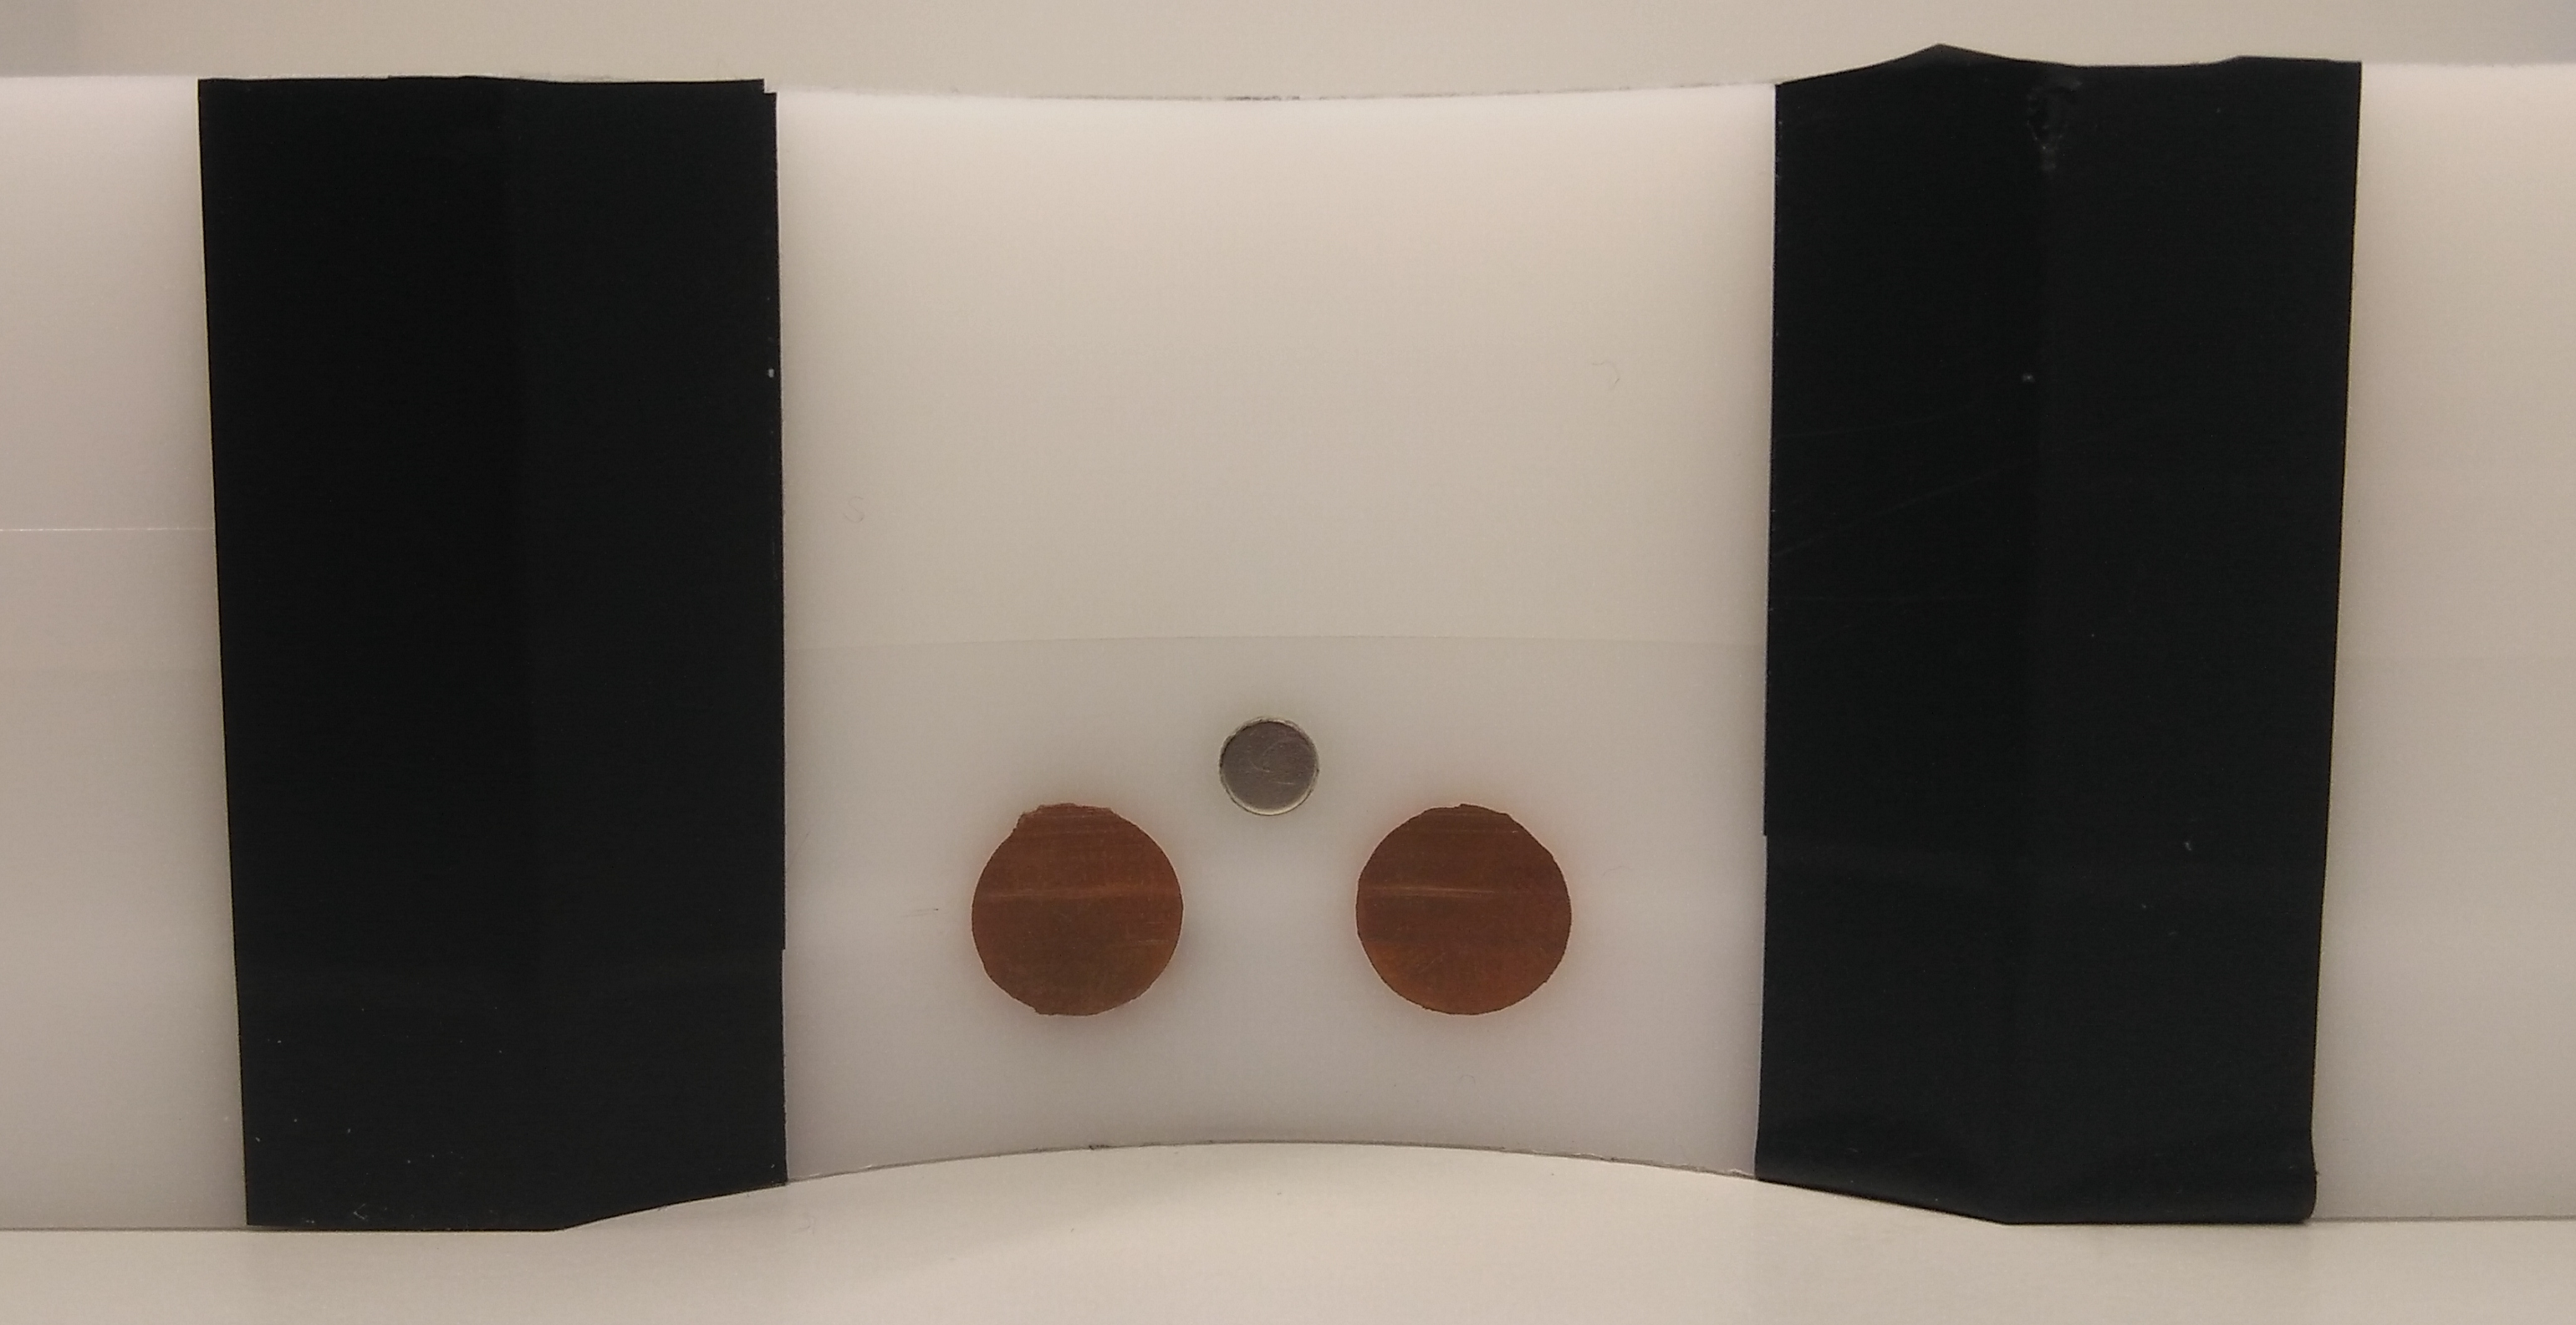
\includegraphics[width=0.6\textwidth]{charging_station_stripes.jpg} 	
		\caption{Ladestation mit Klebestreifen}
		\label{fig:charging_station}
	\end{center}
\end{figure}

Sollte einer der beiden Sensoren 0xFFFF als Wert liefern und der andere einen zu 0xFFFF abweichenden Wert, so steht der AMiRo direkt vor der Wand der Station, muss aber noch in die Richtung des Sensors mit vollem Ausschlag gedreht werden. Da der Magnet der Station eine hohe Anziehung auf die hintere Befestigungsschraube des AMiRos ausübt, ist es nicht möglich den Roboter durch minimales Ansteuern der PWM\footnote{Pulsweitenmodulation}-Steuerung der Motoren zu drehen. Deshalb fährt der Roboter ein kleines Stück aus der Station heraus um sich anschließend in die gegebene Richtung in die Station hinein zu bewegen. 
Wenn ein Sensor einen Wert über 0x4000 und der andere unter 0x4000 liefert, bedeutet dies, dass sich der AMiRo mit einem Abstand vor der Station befindet und seine Position außerdem ein wenig verdreht ist. In dieser Situation muss sich der Roboter in die Richtung des Sensors mit höherem Wert drehen und sich auf die Station zu bewegen. 
Geben beide Sensoren einen Wert über 0x4000 aus, so steht der AMiRo mit Abstand zur Station, muss jedoch nicht gedreht werden. In diesem Fall wird eine gerade Bewegung in Richtung der Station ausgeführt. 
Sollten beiden Sensoren einen Wert unter 0x4000 liefern, so steht der AMiRo in einem zu hohen Abstand zur Ladestation und das Einparken in die Ladestation wird nochmals eingeleitet.

Bevor der Ladevorgang eingeleitet wird, wird die Position des AMiRos nochmals überprüft. Hierfür werden die aktuellen Odometriedaten des Roboters abgerufen und gespeichert. Anschließend wird die PWM-Steuerung der Motoren deaktiviert, was zur Folge hat, dass sich die Reifen frei drehen können. Sollte der AMiRo noch nicht korrekt zur Ladestation ausgerichtet sein, kann die Position des Roboters durch die Wirkung des Magneten auf die Befestigungsschraube verändert werden. Dabei werden die aktuellen Odometriewerte mit den gespeicherten abgeglichen. Sollte sich nach einer Sekunde keine Änderung der Position ergeben haben, so wird eine korrekte Ladeposition angenommen und der Ladevorgang gestartet. Sollte sich die Odometrie verändern, so wird das Justieren nochmals eingeleitet. 




%- Ausgangssituation: AMiRo steht vorwärts in der Ladestation
%- 180$^\circ$ Drehung anhand der Odometrie um die Ladepins zur Station zu richten
%- Justierung der Position anhand der Abstandssensoren und der schwarzen Streifen
%- Abschalten der PWM und Überwachung, ob sich die Position ändert 
%	- Mögliche Fehlerquellen für Positionsänderung: 
%		- AMiRo wird durch den Einfluss des Magnetfeldes auf die Schraube gedreht, da die Position noch nicht gut genug justiert ist
%		- AMiRo wird durch die Federung der Ladepins von der Station abgestoßen, da die Schraube nicht genau vor dem Magneten war und somit die magnetische Kraft nicht groß genug war 

\section[Ansteuern und Überwachen des Ladevorgangs]{Ansteuern und Überwachen des Ladevorgangs\hfill {\normalsize T.M.}}\label{kap:ladevorgang} %TODO: Timo M.

Sobald der AMiRo mit seinen Ladepins zu den Ladekontakten der Ladestation ausgerichtet ist, kann der Ladevorgang eingeleitet werden.
Zunächst wird dem PowerManagement-Board signalisiert, dass der DiWheelDrive-Ladepfad aktiviert werden soll. Nun wird kontrolliert, ob wirklich mindestens 9V an den Pins anliegen und die Akkus aufgeladen werden. Hierfür wird eine kurze Zeit gewartet, da es aufgrund von Signalfilterungen bei der Ermittlung der anliegenden Spannung zu Verzögerungen kommt. Sollten anschließend keine 9V anliegen und die Akkus nicht geladen werden, so wird der Ladevorgang abgebrochen und die Position des AMiRos zur Station wird nochmals justiert.
Liegt die Spannung an und die Akkus werden geladen, so wird während des Ladevorgangs der Status mittels LEDs visualisiert (siehe Abb. \ref{fig:amiro_charging}). 
Währenddessen wird außerdem auf die Odometriedaten des AMiRos geachtet, denn sollte sich etwas an der Position des Roboters ändern, ist nicht mehr sichergestellt, dass alle Pins die Ladekontakte berühren und der Ladevorgang wird abgebrochen. Ein Grund hierfür könnten äußere Einwirkungen wie ein Wackeln am Schaukasten sein.

Nachdem die Akkus des AMiRos voll geladen sind wird der DiWheelDrive-Ladepfad deaktiviert, die PWM-Steuerung aktiviert und der Roboter fährt ein Stück aus der Ladestation heraus.

\begin{figure}[]
	\begin{center}
		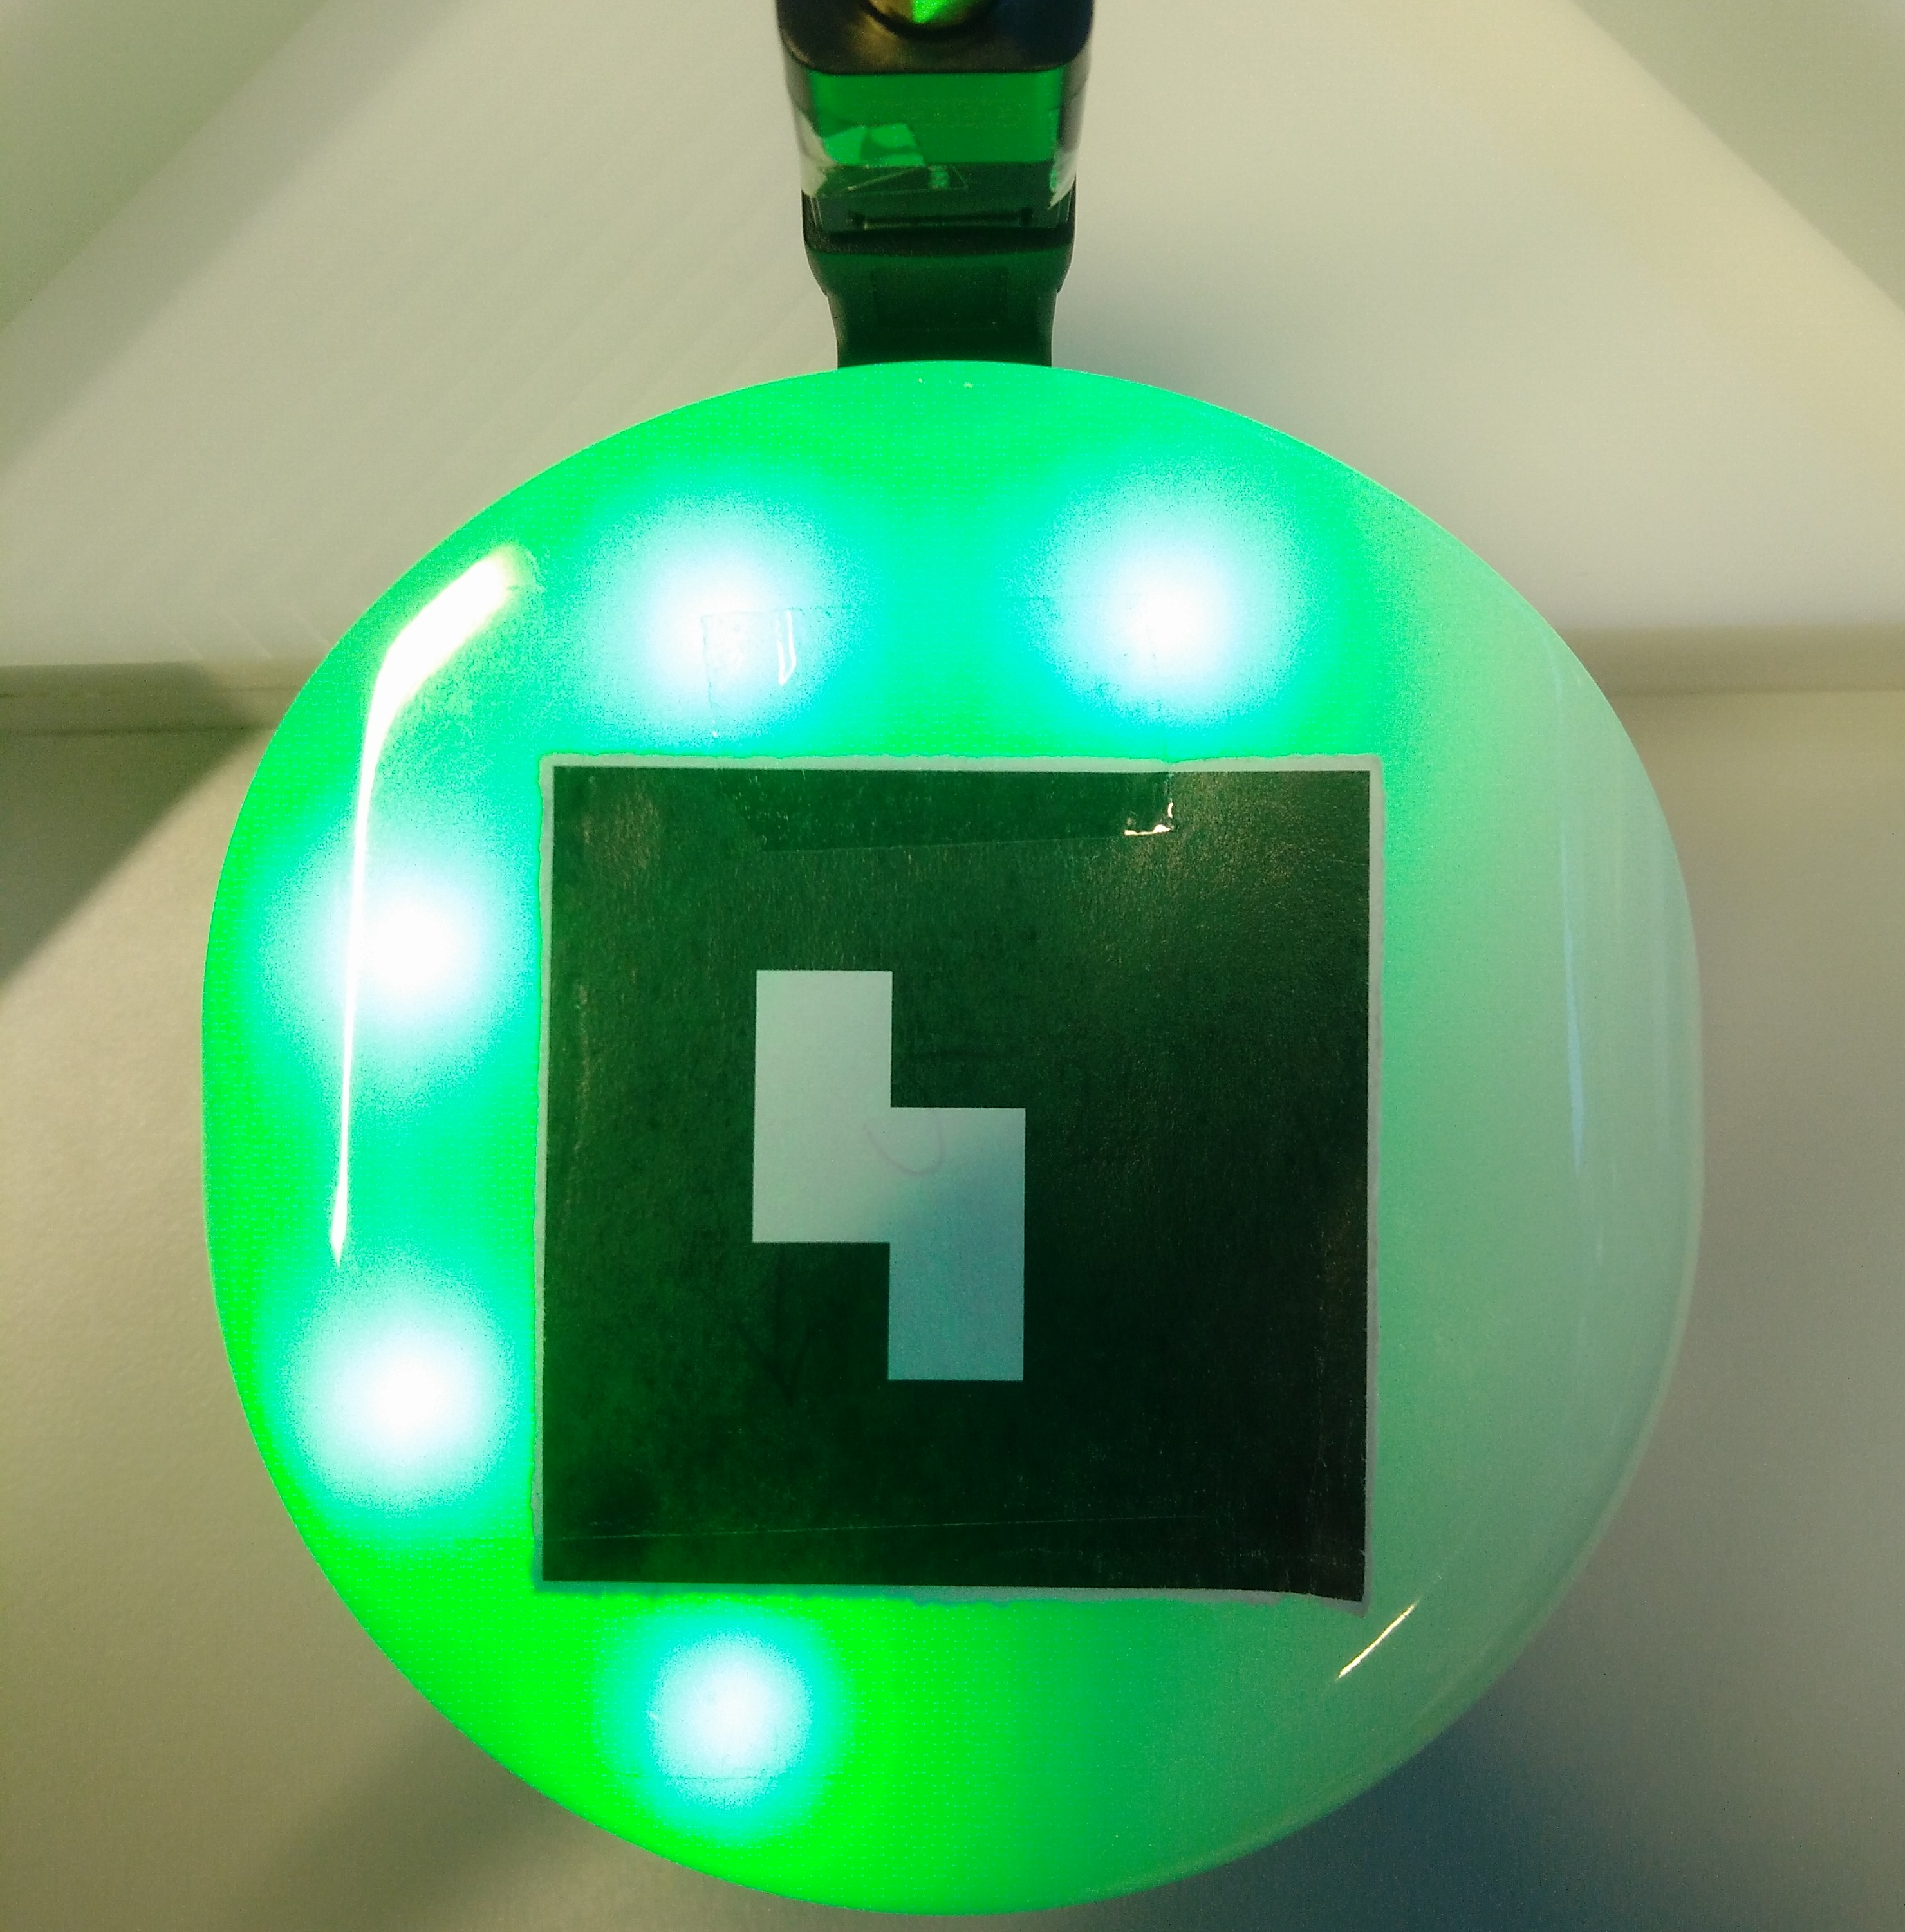
\includegraphics[width=0.5\textwidth]{AMiRo_charging.jpg} 	
		\caption{Ladeanimation}
		\label{fig:amiro_charging}
	\end{center}
\end{figure}



%- Aktivieren des DiWheelDrive-Board Ladepfades (+ kurzes Abwarten)
%- Kontrolle, ob mehr als 9V anliegen (wenn nicht -> Position erneut justieren)
%- Überwachen des Ladevorgangs
%	- Auslesen der Ladestatus der Akkus (\% und Zeit bis geladen)
%	- Überwachen der Odometrie 
%		- falls sich der AMiRo aufgrund von äußeren Einwirkungen bewegen sollte -> Abbruch des Ladevorgangs und Position erneut justieren


\chapter{Fussballszenario} \label{kap:Fussballszenario} %TODO: Besseren Kapiteltitel

\section[Szenario Koordination]{Szenario Koordination\hfill {\normalsize H.O.}}

Die Szenario Koordination umfasst sowohl das Verhalten der einzelnen AMiRos, kooperative Elemente zwischen verschiedenen AMiRos, als auch die Kommunikation mit dem Host-PC. Der Entwurf dieser drei Themenbereiche soll im folgenden kurz vorgestellt und begründet werden:

Um ein bestimmtes Verhalten zu zeigen, müssen die AMiRos selbst zunächst über einen Satz einzelner Fähigkeiten verfügen. Ein komplexeres Verhalten entsteht dann aus der Kombination der einzelnen Fähigkeiten, indem diese sequenziell oder parallel miteinander kombiniert werden. Denkbar wäre ebenso die Realisierung einer Verhaltenshierarchie, in der sich einzelne Verhaltensweisen beeinflussen und sich gegenseitig unterdrücken oder verstärken können. Ein solcher Ansatz wird näher in \cite{Brooks:1986} beschrieben.

Da das Szenario in seiner Komplexität jedoch noch begrenzt ist und kein vollständig generisches Verhalten implementiert werden musste, wurde die Umsetzung im Projektkontext durch einen endlichen Automaten / eine (Finite-)State-Machine realisiert. Die Zustände stellen einzelne Verhaltensweisen des Roboters dar und durch bestimmte Nachrichten (Events) kann zwischen ihnen gewechselt werden.

Das Verhalten einzelner AMiRos wird erweitert durch kooperative Fähigkeiten und die Möglichkeit der Kommunikation durch einen festgelegten Befehlssatz. Kann beispielsweise ein AMiRo während einer Spielaktion den Ball nicht lokalisieren, kann er eine Nachricht an den anderen AMiRo schicken, woraufhin dieser sich dann ein Stück bewegt, um die Sicht auf den Ball freizugeben.

Zusätzlich besteht die Möglichkeit für die AMiRos mit dem Host-PC zu kommunizieren, welcher an Hand eines Kamerabildes und zusätzlicher Bildverarbeitungslogik das Spielgeschehen verfolgen, interpretieren und steuern kann. Dies erlaubt außerdem eine Benutzerinteraktion, um das Spiel zu starten, zu pausieren oder zu unterbrechen. In der derzeitigen Realisierung übermittelt der Host-PC außerdem noch den Status des Spielballs, also ob dieser in Bewegung ist oder ruht. Diese Information wird von den AMiRos verwendet, um eigenständig zu bestimmen, welcher AMiRo gerade am Zug ist.

\vfill

\section[Kommunikation per RSB und Spread]{Kommunikation per RSB und Spread\hfill {\normalsize H.O.}}
Damit die AMiRos untereinander kommunizieren können, wurde eine Publish-Subscribe Architektur basierend auf der RSB Middleware aufgesetzt und anstatt einer einfachen Socket-Transport Lösung wurde auf das etwas komplexere Spread Toolkit zurückgegriffen (siehe RSB Konfigurationsdatei im Anhang \ref{sec:rsb-config}).

Die Publish-Subscribe Architektur bietet den Vorteil der asynchronen Kommunikation, die im Zusammenspiel mit einer State-Machine besonders praktisch ist. Die State-Machine muss nicht auf explizit auf Antworten warten, sondern kann beliebig weiterlaufen und schaut in jedem Zyklus, ob neue Nachrichten empfangen wurden. Zudem bietet sie den Vorteil, dass sehr leicht Software-Komponenten hinzugefügt und an die bestehende Kommunikation angeschlossen werden können (vgl.\cite{Siciliano:2007}).

Jeder AMiRo (und auch der Host-PC) hat also eine bestimmte Anzahl an Empfängern (Listener) und Sendern (Publisher) um Nachrichten in bestimmten Geltungsbereichen (Scopes) zu empfangen oder zu senden. Als Nachrichten werden der Einfachheit halber einfache Strings versendet, die dann beim Empfänger geparst werden können. Das Debugging während der Entwicklung wurde so vereinfacht, allerdings hat dieser Ansatz auch Nachteile: Zum einen müssen die Listen an Strings auf Empfänger und Senderseite immer gepflegt werden, damit sie identisch sind und ein zuverlässiges Parsen erlauben. Zum anderen bieten gekapselte Nachrichten mehr Typensicherheit und ggf. auch die Option zusammengehörige Informationen zu kapseln. Im Umfang des Projekt war die Wahl lediglich einfach Strings zu übertragen durchaus ausreichend, die Lösung skaliert aber nicht zwingend für größere Projekte.

Das Spread Toolkit hilft dabei einen Nachteil der allgemeinen Publish-Subscriber Architektur zu beseitigen: Die Kommunikation beruht nicht auf einem zentralen Endpunkt, der die gesamte Kommunikation steuert, sondern jeder Spread-Daemon überwacht die Verbindungen zu allen anderen Endpunkten und hält diese so aufrecht (vgl.\cite{Siciliano:2007}). So kann auch bei kurzzeitigen Verbindungsabbrüchen sichergestellt werden, dass die Verbindung automatisch wiederhergestellt wird. Auf Programmebene  muss so weniger Overhead für die Sicherstellung der Verbindung implementiert werden und der Code bleibt einfacher und somit besser wartbar.

Neben der Plattform-übergreifenden Kommunikation werden RSB und Spread zusätzlich auch für Interprozess-Kommunikation auf den AMiRos und auf dem Host-PC eingesetzt. Wie in Abb. \ref{fig:spread} zu sehen ist, laufen auf beiden AMiRos die drei gleichen Softwarekomponenten. Die State-Machine (\texttt{FSM}) steuert das Verhalten und die Kommunikation. Die \texttt{locateAndShoot} Komponente stellt die Verhaltenseinheiten für das Szenario zur Verfügung und die \texttt{SearchCharging} Komponente erlaubt aus dem Szenario aus die Lokalisation und das Anfahren an die Ladestation. Diese drei Komponenten kommunizieren über den internen Spread, der auf der internen Localhost Schnittstelle auf dem Port 4806 läuft (siehe dazu auch Anhang \ref{sec:spread-config}).

Die Kommunikation zwischen den AMiRos selbst und dem Host läuft über einen weiteren Spread-Daemon, der mit einer anderen Konfiguration geladen wird, die W-LAN Schnittstelle nutzt und auf Port  4803 hört und sendet (siehe ebenfalls Abschnitt \ref{sec:spread-config}).

Die W-LAN Verbindung wurde durch einen eigenen Router realisiert und erlaubt so die feste Adresszuweisung für die drei Endpunkte, damit die Spread-Konfiguration darauf zurückgreifen kann. Die Einzelheiten können der W-LAN Konfiguration im Anhang (Abschnitt \ref{sec:wlan-config}) entnommen werden.
\begin{figure}[H]
	\begin{center}
		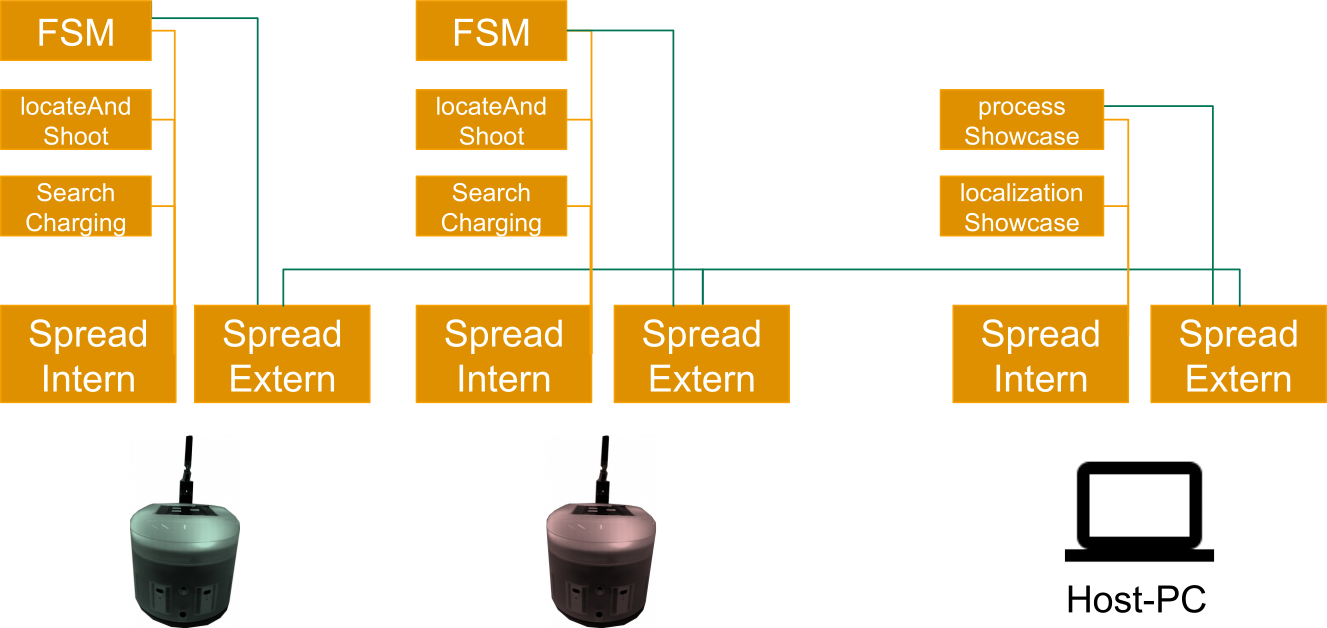
\includegraphics[scale=.65]{spread_communication.png} 	
		\caption{Spread-Kommunikation}
		\label{fig:spread}
	\end{center}
\end{figure}


\subsection[Finite-State-Machine]{Finite-State-Machine\hfill {\normalsize H.O.}}
Die State-Machine regelt das Verhalten der einzelnen AMiRos. Jedes Verhalten wird in kleinstmögliche Einheiten unterteilt, die dann einzeln angesprochen und überall wiederverwendet werden können. Nach der Initialisierung aller RSB-Komponenten und Variablen wird im Programm die State-Machine gestartet.

Solange kein Fehler auftritt, bleibt das Programm immer innerhalb der State-Machine und wechselt den aktuellen Zustand nur auf Grund externer Nachrichten, die in Form von RSB Events oder CAN Messages eingehen können. Extern beschreibt also in diesem Zusammenhang sowohl die anderen Programmkomponenten die auf dem AMiRo laufen, als auch RSB Events von einem anderen AMiRo oder dem Host-PC und CAN Nachrichten vom Mikrocontroller.

Einzelne Zustände haben auch direkte Anweisungen, die den aktuellen Zustand wechseln können, dies soll eine Kapselung der einzelnen Verhaltenseinheiten unterstützen und erlaubt so zukünftige Änderungen oder Erweiterungen leichter durchführen zu können.

Die State-Machine selbst ist in Abb. \ref{fig:fsm-amiro} dargestellt. Nach dem Start ist zunächst der \texttt{idle} Zustand aktiv. Dieser wartet lediglich auf Kommandos und stellt sicher, dass sich der AMiRo nicht bewegt, sondern ruhig auf seiner Position abwartet.

Um das Spiel zu starten, muss eine Nachricht vom Host-PC an die AMiRos geschickt werden.Der aktuelle Zustand wechselt dann auf \texttt{startScenario}. Hier können Initialisierungen vorgenommen werden, die notwendig sind, damit der Roboter das Spiel antreten kann. In der derzeitigen Implementierung werden beispielsweise die Teamfarben auf den oberen LEDs des AMiRos gesetzt. Eine mögliche Erweiterung des Szenarios wäre beispielsweise, dass die Spieler auch bestimmte Positionen auf dem Spielfeld einnehmen.

Ist die Initialisierung abgeschlossen, wechselt die State-Machine in den \texttt{ready} Zustand. In diesem Zustand bleibt die FSM solange, bis der Host-PC das Spiel offiziell startet, doch abbricht oder bis die Ladestrategie das Ladeverhalten anstößt.

Wird das Spiel gestartet, ist der \texttt{waitForTurn} State aktiv. Dieser wartet im Normalfall auf die Nachricht eines anderen AMiRos, der seinen Spielzug abgeschlossen hat und somit das Handle an ihn selbst übergibt. Beim Spielstart hingegen versendet der Host-PC einmalig ein Event mit entsprechendem Inhalt und definiert so, welche Roboter beginnen darf. Im normalen Spielverlauf kann es auch passieren, dass der AMiRo dem Gegner die Sicht auf den Ball verdeckt. Signalisiert der Gegner dies durch eine Nachricht, wechselt die State-Machine in den \texttt{moveFromBall} State, sendet dort eine Nachricht an die \texttt{locateAndShoot} Anwendung und wechselt dann wieder zurück in den \texttt{waitForTurn} Zustand. Gleichzeitig wird eine Bestätigungsnachricht an den Gegner verschickt um zu signalisieren, dass die Neupositionierung abgeschlossen ist.

Ist der AMiRo selbst an der Reihe, um seinen Spielzug zu machen, beginnt er damit im \texttt{localizeBall} State. Er versucht den Ball zu lokalisieren und wechselt bei erfolglosem Versuch in den \texttt{waitForOtherAmiroMove} Zustand, in dem eine Nachricht an den Gegner geschickt wird, damit dieser sich bewegt. Nach Bestätigung des Gegners, dass dieser seine Position geändert hat, wechselt die FSM wieder in den \texttt{localizeBall} Zustand und versucht erneut die Lokalisierung des Balls. Bei Erfolg wird dann zu \texttt{moveToBall} gewechselt.

Die folgenden Zustände verlaufen sequenziell und können daher zusammenfassend beschrieben werden:
\texttt{moveToBall}, \texttt{findGoal}, \texttt{moveToShootingPosition}, \texttt{shootBall}. Jeder dieser Zustände verschickt ein Event an das \texttt{locateAndShoot} Programm, wartet auf erfolgreiche Rückmeldung und wechselt dann in den jeweils nachfolgenden State. Wie auch in den meisten Zuständen zuvor, gibt es zusätzlich noch die Möglichkeit, dass das Spiel abgebrochen wird oder der AMiRo laden muss. Dann wird jeweils in den \texttt{cancelScenario} oder in den \texttt{moveToEdge} State gewechelt.

Nachdem der Ball vom Roboter geschossen wurde, muss zunächst auf eine Bestätigung vom Host-PC gewartet werden, bis der Ball sich nicht mehr bewegt. Erst dann soll das Handle an den anderen AMiRo übergeben werden. Der Host-PC sendet allerdings kontinuierlich ein Signal aus, solange sich der Ball bewegt, die State-Machine wartet sicherheitshalber mehrere Durchgänge in denen keine Nachricht vom Host-PC empfangen werden darf, die eine Ballbewegung signalisiert. Erst dann wird das Handle im nachfolgenden State \texttt{giveHandleToOtherAmiro} übergeben. In diesem Zustand ist ein Hand-Shaking Mechanismus eingebaut, um sicherzustellen, dass der Gegner das Handle auch empfangen hat. Ist das der Fall, wird wieder zurück in den \texttt{waitForTurn} Zustand gewechselt.

Auch das Ladeverhalten wird aus State-Machine Sicht in mehrere Schritte unterteilt und erlaubt so eine gewisse Flexibilität. Gestartet wird das Ladeverhalten durch den \texttt{moveToEdge} State, der den Roboter aus dem Spielgeschehen heraus lenken soll, bis er die nächste Kante gefunden hat.

Ist er dort angekommen, wechselt er in den \texttt{waitingAtEdge} Zustand. Je nach dem ob die Ladestation gerade frei ist, kann die FSM dann direkt in den nächsten Zustand übergehen oder muss dort solange warten, bis die Ladestation frei wird.

Im \texttt{moveToCharging} Zustand startet der AMiRo eine Kantenverfolgung und versucht dann an Hand bestimmter Merkmale die Ladestation zu lokalisieren, indem er entsprechende RSB Events an die SearchCharging Anwendung sendet.

Ist er an der Ladestation angekommen, wechselt die State-Machine in den\linebreak \texttt{moveIntoStation} State und kommuniziert dann über CAN Nachrichten mit den Mirkocontroller Schnittstellen. Wird ein erfolgreiches Andocken zurückgemeldet, wird dann (ebenfalls über CAN) das eigentliche Laden gestartet. Der Roboter lädt dann in der Regel vollständig auf, es sei denn er empfängt zwischendurch Notrufsignale von einem anderen AMiRo der einen kritischen Ladezustand erreicht hat. 

\subsection[Ladestrategie]{Ladestrategie\hfill {\normalsize H.O.}}
Während des Szenarios ist es für die Roboter wichtig, ihren eigenen Ladezustand zu überwachen und beim Überschreiten gewisser Grenzwerte ein bestimmtes Verhalten auszulösen.

Der aktuelle Ladezustand kann wird bei jedem Durchlauf der FSM über den CAN Bus abgefragt und überprüft. Die genaue Ladestrategie wird in Abb. \ref{fig:charging-strategy} verdeutlicht. Fällt die Ladekapazität unter 10\%  wird zunächst überprüft, welchen Ladezustand der andere AMiRo aktuell hat. Liegt dieser unter 15\%, wird das Ladeverhalten gestartet. Fällt die eigene Ladekapazität unter 5\% wird das Ladeverhalten ebenfalls ausgelöst, unabhängig vom Ladezustand des anderen AMiRos. Wird dann eine weitere Grenze von 2\% unterschritten, wird zusätzlich eine Art Notrufsignal vom AMiRo gesendet. Dieses Signal veranlasst einen anderen Roboter, welcher gerade die Ladestation blockiert, aber schon ein bestimmtes Ladelevel erreicht hat, seinen Ladevorgang abzubrechen und die Ladestation frei zu machen.

\begin{figure}[H]
	\begin{center}
		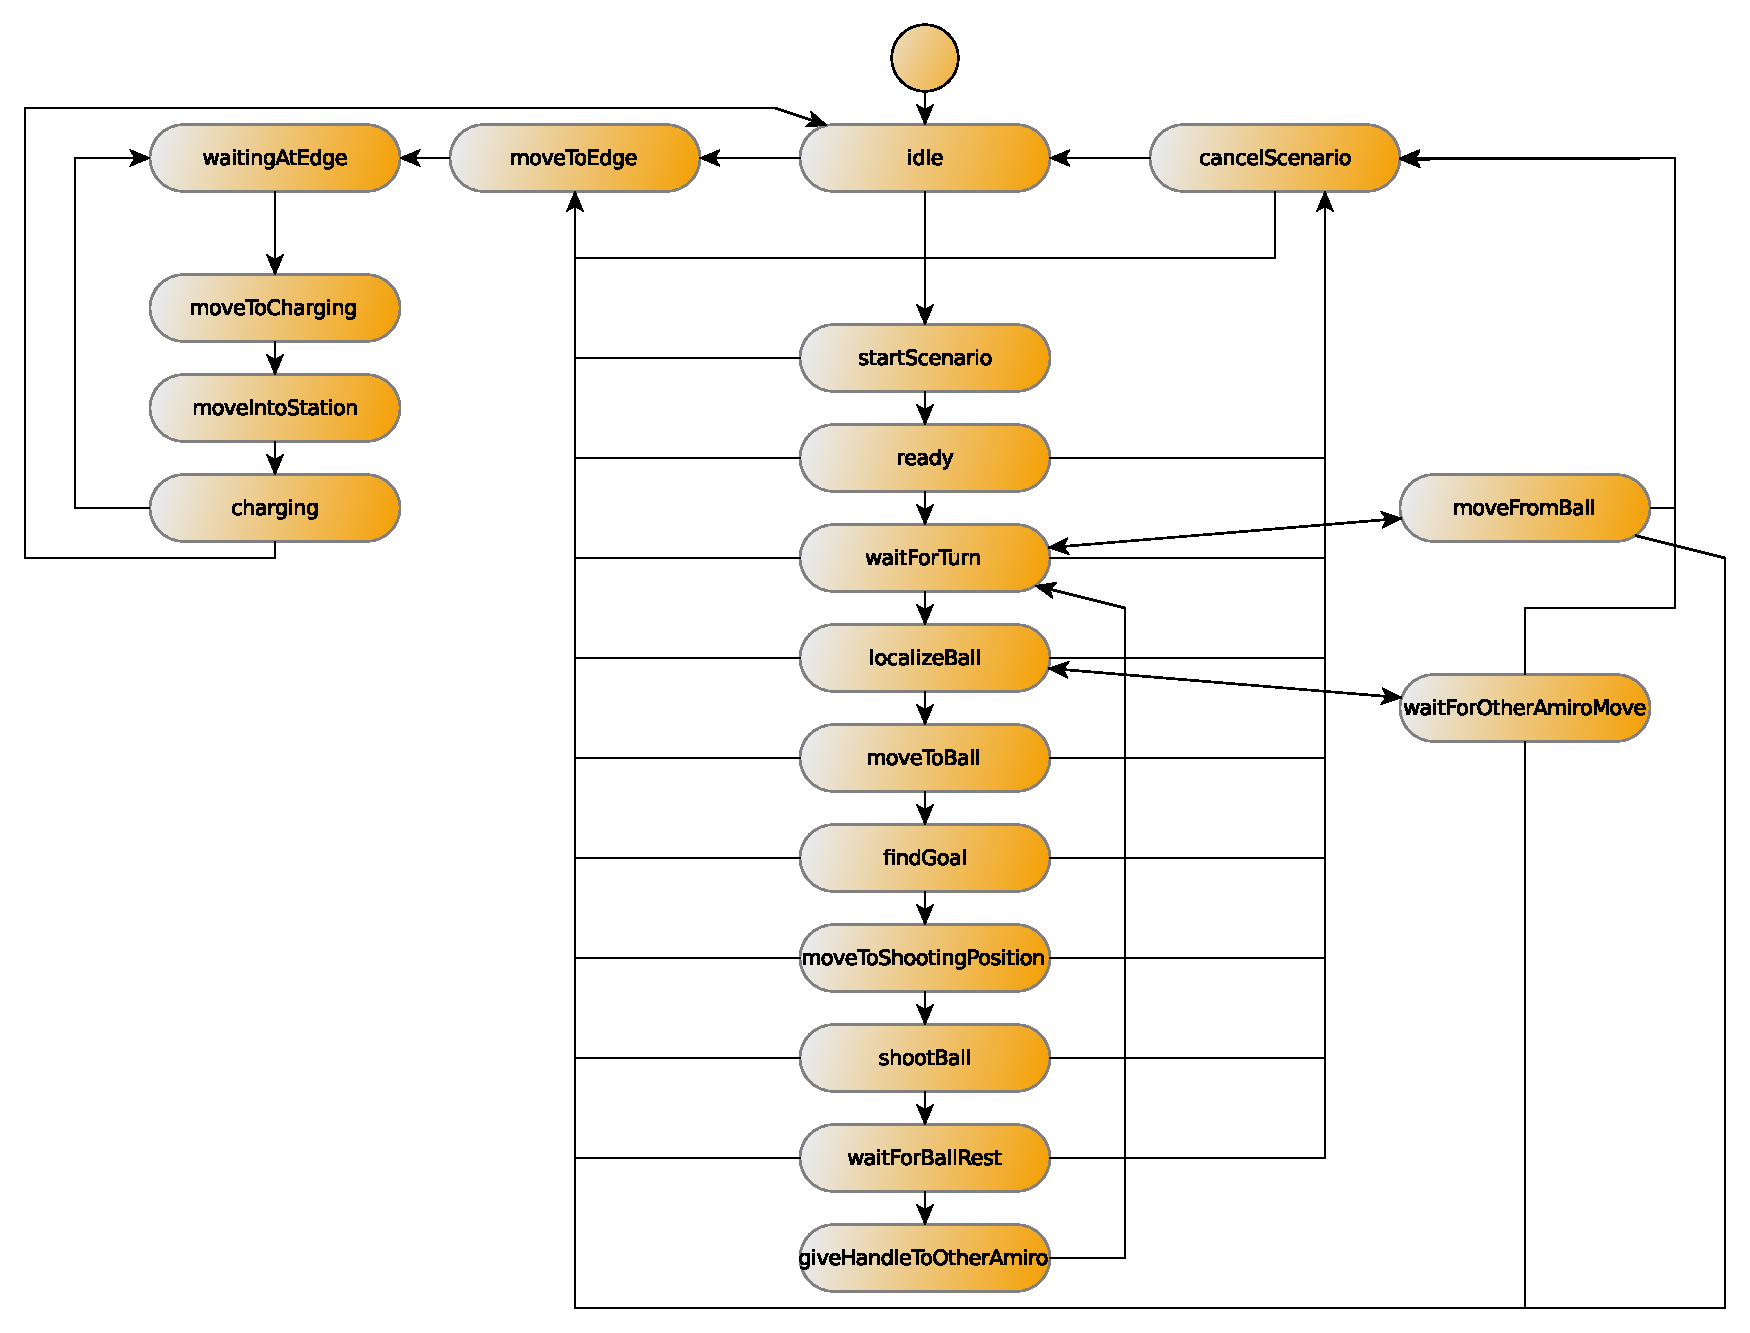
\includegraphics[scale=.55]{Final_FSM_AMiRo.pdf} 	
		\caption{Finite-State-Machine}
		\label{fig:fsm-amiro}
	\end{center}
\end{figure}
\begin{figure}[H]
	\begin{center}
		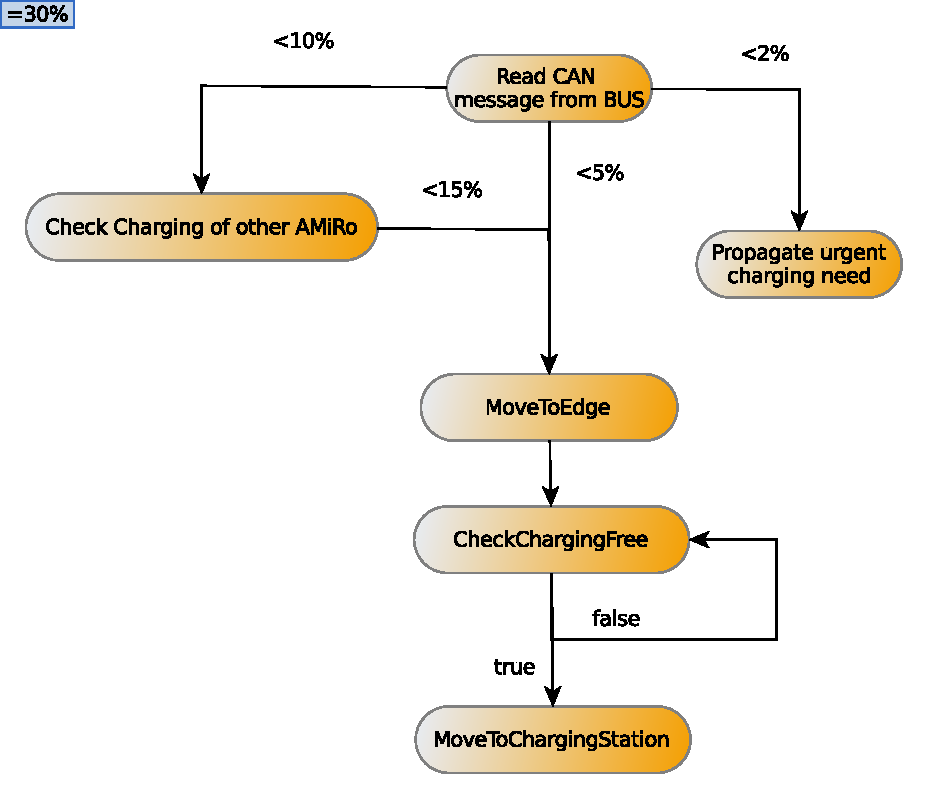
\includegraphics[scale=.50]{Charging_Strategy.pdf} 	
		\caption{Ladestrategie}
		\label{fig:charging-strategy}
	\end{center}
\end{figure}


\section[Realisierung der einzelnen Spielelemente]{Realisierung der einzelnen Spielelemente\hfill {\normalsize ?.?.}}%TODO: Besseren Sectiontitel

\subsection[Lokalisation des Balls]{Lokalisation des Balls\hfill {\normalsize J.E.}} %TODO: Julian E.

\subsection[Anfahren des Balls]{Anfahren des Balls\hfill {\normalsize J.E.}} %TODO: Julian E.

\subsection[Lokalisation des gegnerischen Tores]{Lokalisation des gegnerischen Tores\hfill {\normalsize T.M.}} %TODO: Timo M.
- Rotation um eigene Achse zur Lokalisation des Tores
- Lokalisation Anhand von Blobb-Detektion 
- Wenn ein einzelner Pfosten im Bild vorhanden ist - bereits gedrehten Winkel + zusätlichen Winkel vom Mittelpunkt des Bildes zum Pfosten speichern
- Wenn beide Pfosten im Bild vorhanden sind - bereits gedrehten Winkel + zusätlichen Winkel vom Mittelpunkt des Bildes zum Tormittelpunkt speichern und Rotation beenden
- Drehung zum Ball durchführen, um diesen wieder vor sich zu haben

\subsection[Schussposition anfahren]{Schussposition anfahren\hfill {\normalsize T.M.}} %TODO: Timo M.
- Je nach Winkel zum Tor entscheiden, ob der Ball links- oder rechtsseitig umfahren werden soll
- 90$^\circ$ Drehung zu der gegebenen Seite 
- Umfahren des Balles bis vorher berechneter Winkel zum Tor erreicht ist
	- Bei einem Hindernis wird das Umfahren des Balles gestoppt
- 90$^\circ$ Drehung zum Ball
- Überprüfung, ob sowohl Ball als auch das Tor im Bild zu sehen ist 
	- Ist dies der Fall -> feinjustierung der Schussposition 

\subsection[Schießen]{Schießen\hfill {\normalsize T.M.}} %TODO: Timo M.
- Überprüfen der seitlichen vorderen Abstandssensoren ob eine Wand detektiert wird
	- Sollte eine Wand auf einer Seite detektiert werden -> Angedrehter Schuss mit Drehung des AMiRos weg von der Wand
- Schießen des Balles durch kurzes Ansteuern beider Motoren 

\subsection[Beiseite Fahren]{Beiseite Fahren\hfill {\normalsize J.E.}} %TODO: Julian E.

\subsection[Torjubel]{Torjubel\hfill {\normalsize A.G.}} %TODO: Andi G.

\subsection[Spieltracking]{Spieltracking\hfill {\normalsize J.D.}} %TODO: Julian D.

\subsection[Spielfeldbestimmung mit dem AR Toolkit]{Spielfeldbestimmung mit dem AR Toolkit\hfill {\normalsize J.D.}} %TODO: Julian D.

\subsection[Extraktion wichtiger Spielelemente mit Bildverarbeitungsmethoden]{Extraktion wichtiger Spielelemente mit Bildverarbeitungsmethoden\hfill {\normalsize J.D.}} %TODO: Julian D.

\subsection[Benutzerinteraktion mit AR Markern]{Benutzerinteraktion mit AR Markern\hfill {\normalsize J.D.}} %TODO: Julian D.

\subsection[Spielkoordination]{Spielkoordination\hfill {\normalsize J.D.}} %TODO: Julian D.

\subsection[Grafische Darstellung der Spielstatus]{Grafische Darstellung der Spielstatus\hfill {\normalsize J.D.}} %TODO: Julian D.


% ...

\appendix
\listoffigures
%\lstlistoflistings
%\cleardoublepage
%\addcontentsline{toc}{chapter}{Literaturverzeichnis}
%\bibliographystyle{alpha}
%\bibliographystyle{geralpha} % benoetigt packet bibgerm
%\bibliography{literatur}
\printbibliography

\chapter{Anhang}

\section{Spread Konfiguration}
\label{sec:spread-config}

AMiRo Kommunikation mit anderen AMiRos / Host:\\
(File=spreadShowcase.conf)

\lstset{language=bash}
\begin{lstlisting}
Spread_Segment  10.0.0.255:4803 {
	# amiro27
	stick1          10.0.0.201
}

Spread_Segment 10.0.0.255:4803 {
	# amiro23    
	stick0          10.0.0.202
}

Spread_Segment  10.0.0.255:4803 {
	lagomera        10.0.0.200
}
\end{lstlisting}

Interprozesskommunikation AMiRo:\\
(File=spreadShowcaseAMiRoInternal.conf)

\begin{lstlisting}
Spread_Segment  127.0.0.255:4806 {
	localhost               127.0.0.1
}
\end{lstlisting}


\section{RSB Konfiguration}
\label{sec:rsb-config}
AMiRo RSB Konfiguration\\
(File=rsb.conf)

\begin{lstlisting}
[plugins.cpp]
load    = rsbspread
[transport.inprocess]
enabled = 0
[transport.socket]
enabled = 0
[transport.spread]
enabled = 1
host    = 127.0.0.1
port    = 4806
\end{lstlisting}


\section{W-LAN Konfiguration}
\label{sec:wlan-config}
ASUS Router Konfiguration:\\
SSID: aseshowcase\\
PASS: aseshowcase\\

IP Adressen:\\
lagomera 10.0.0.200\\
stick1 10.0.0.201\\
stick0 10.0.0.202\\

Allgemeine Konfiguration des Connman Netzwerkmanagers:\\
/var/lib/connman/<SSID>-psk.config
\begin{lstlisting}
[service_wifi_<hash>_managed_psk]
Type       = wifi
Name       = <SSID>
Passphrase = <passphrase>
\end{lstlisting}

Spezifische Konfigurationen der beiden AMiRos:\\
/var/lib/connman/aseshowcase-psk.config

stick1:
\begin{lstlisting}
[service_wifi_wifi_74da380645e3_
61736573686f77636173655f3547_managed_psk]
Type       = wifi
Name       = aseshowcase
Passphrase = aseshowcase
Hidden     = false
IPv4       = dhcp
IPv6       = off
\end{lstlisting}

stick0:
\begin{lstlisting}
[service_wifi_wifi_74da380645f6_
61736573686f77636173655f3547_managed_psk]
Type       = wifi
Name       = aseshowcase
Passphrase = aseshowcase
Hidden     = false
IPv4       = dhcp
IPv6       = off
\end{lstlisting}



%%
%\cleardoublepage
%\thispagestyle{empty}
%\subsection*{Erklärung}
%Ich versichere, dass ich die vorliegende wissenschaftliche Arbeit 
%selbstständig verfasst und keine anderen als die angegebenen
%Hilfsmittel verwendet habe. Die Stellen der Arbeit, die anderen 
%Werken dem Wortlaut oder dem Sinn nach entnommen sind, wurden 
%unter Angabe der Quelle als Entlehnung deutlich gemacht. Das 
%Gleiche gilt auch für beigegebene Skizzen und Darstellungen. Diese 
%Arbeit hat in gleicher oder ähnlicher Form meines Wissens nach 
%noch keiner Prüfungsbehörde vorgelegen.
%
%\thesisDate
%
%~
%
%~
%
%\thesisAuthor

\end{document}
